\documentclass{article}
\usepackage[utf8]{inputenc}
\usepackage{textcomp}
\usepackage{gensymb}
\usepackage{graphicx}
\usepackage{multicol}
\usepackage{amsmath}
\usepackage{amssymb}
\usepackage{physics}
\usepackage{hyperref}
\usepackage{cancel}
\usepackage{scalerel}

\def\msquare{\mathord{\scalerel*{\Box}{gX}}}

\graphicspath{ {./chap5images/} }

\oddsidemargin=-.3in
\evensidemargin=-.5in
\textwidth=7in
\topmargin=-1in
\textheight=10in

\parindent=.2in
\pagestyle{plain}

\title{\textbf{The Rational Numbers} \\ \large Math 1 - Chapter 5}
\author{Theo Rode}
\date{}

\begin{document}

\maketitle 

It is time to talk about more numbers! I would say these are new to you, but we have actually already explored these types of numbers. 
% I will leave the suspense for what these numbers are until later on and for now, I am going to talk about something you have already seen before: decimals. 

% Now decimals aren't necessarily rational numbers, they are just a way of counting quantities less than 1. They are very similar to how ``normal'' numbers work. As you know, with the number: 
% \[ 32014 \]

% We can rewrite this as saying there are: 
% \[ 4 \cdot 1 \]
% \[ 1 \cdot 10  \]
% \[ 0 \cdot 100 \]
% \[ 2 \cdot 1000 \]
% \[ 3 \cdot 10000 \]

% We start on the right, and we say that the first single digit on the right represents that many of the number 1. In this case, four ones. 
% The next digit then represents how many 10s there are, in this case 1. And then one more to the right represents 10 times 10. And then 10 times 10 times 10. And then 10 times 10 times 10 times 10. And so on. 

% All of these calculated numbers are added together to get the full number: 
% \[ 4 \cdot 1 + 1 \cdot 10 + 0 \cdot 100 + 2 \cdot 1000 + 3 \cdot 10000 \]
% \[ = 4 + 10 + 2000 + 30000 \]
% \[ = 32014 \]

% Pretty simple. You have been doing this forever. With decimals, we add this little dot to the right of the ones place and then put more digits to the right of that! 
% \[ 32014.6573 \]

% With this new number we have the same numbers to the left of the decimal point: 
% \[ 4 \cdot 1 \]
% \[ 1 \cdot 10  \]
% \[ 0 \cdot 100 \]
% \[ 2 \cdot 1000 \]
% \[ 3 \cdot 10000 \]

% But with these new, smaller digits to the right of the decimal point. Each of these represents a quantity less than 1. In fact, much like how we were multiplying by 10 going to the left, we are now undoing multiplying by ten going to the right. 
% If you remember, this means multiplying by the inverse of 10:
% \[ \frac{1}{10} \]

% So for the first digit to the right of the decimal point, for this number, we have:
% \[ 6 \cdot (1 \cdot \frac{1}{10}) \] 

% Or in words, six of the number that is 10 times \textbf{smaller} than 1. What you might also realize is that this number that is 10 times smaller than 1 is actually just:
% \[ \frac{1}{10} \]

% Because the multiplicative identity, 1, multiplied by anything is just that anything. That is interesting. But we will come back to that. 

% Every decimal place to the right of the decimal point represents a number ten times less. So in the end, all the decimal places come out to:
% \[ 6 \cdot \left(\frac{1}{10}\right) \]
% \[ 5 \cdot \left(\frac{1}{10} \cdot \frac{1}{10}\right) \]
% \[ 7 \cdot \left(\frac{1}{10} \cdot \frac{1}{10} \cdot \frac{1}{10}\right) \]
% \[ 3 \cdot \left( \frac{1}{10} \cdot \frac{1}{10} \cdot \frac{1}{10} \cdot \frac{1}{10} \right) \]

% We now add these all together to get the number we desire: 
% \[ 1 \cdot 10 + 0 \cdot 100 + 2 \cdot 1000 + 3 \cdot 10000 + 4 \cdot 1 + 6 \cdot \left(\frac{1}{10}\right) + 5 \cdot \left(\frac{1}{10} \cdot \frac{1}{10}\right) + 7 \cdot \left(\frac{1}{10} \cdot \frac{1}{10} \cdot \frac{1}{10}\right) + 3 \cdot \left( \frac{1}{10} \cdot \frac{1}{10} \cdot \frac{1}{10} \cdot \frac{1}{10} \right)\]
% \[ = 32014.6573 \]

% And this is how we typically represent numbers. We know that 100 is greater than 10 and we know that 0.03 is less than 1. We can represent a whole host of numbers using this technique. 

You ready for it? This is a rational number: 
\[ 1 \]

Oh. So it is literally the same as an integer? Why does it have a different name? 

Well, 1 is a rational number, but there is more than just 1. There is: 
\[ \frac{1}{10} \]

Yes. We explored the possibility of fractions being numbers earlier and in fact, they are rational numbers!
So then, what does the value $\frac{1}{10}$ represent? Well, we know that multiplying this number by another number ``undos'' multiplying by 10. And if we multiply this by 1: 
\[ 1 \cdot \frac{1}{10} \]

Well we know that 1 is the multiplicative identity, so this is just: 
\[ \frac{1}{10} \]

This would indicate that if we multiplied this rational number by 10, we would get 1. Meaning, that this represents a value that is 10 times smaller than 1! 

To further convince you of this, consider multiplying this value by 10: 
\[ \frac{1}{10} \cdot 10 \]

Because we know multiplying by the inverse grants us the identity, this must be: 
\[ \frac{1}{10} \cdot 10 = 1 \]

Meaning that it does in fact take 10 groups of $\frac{1}{10}$ to get to the number 1! 

It can sometimes be hard to imagine a number less than 1. What does it mean to have $\frac{1}{10}$ stones? That is even a weird sentence to say \footnote{This is especially because you say $\frac{1}{10}$ as ``one-tenth'' so the grammar isn't even right.} One thing that can help is representing these numbers like so: 
\begin{center}
    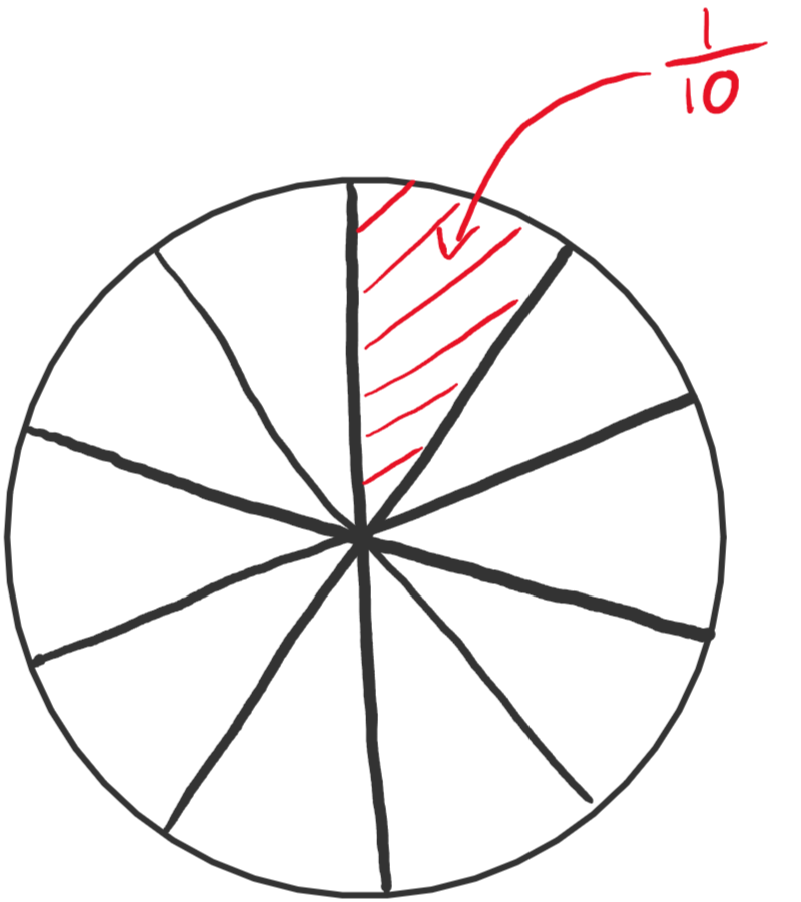
\includegraphics[scale=0.5]{chapter5_draw1.png}
\end{center}

I mean the drawing could use some improvement (I am here to talk about math not art), but the idea is what is important. You want to look at splitting the object into 10 parts and, for $\frac{1}{10}$, taking 1 of those parts. You can imagine adding together these ``parts'' or taking parts of the parts ($\frac{1}{10} \cdot \frac{1}{10}$).

But this begs the question: what if we have more than just 1 part of something? Say we have 2 parts or 3 parts? What does that number look like? 
Well, it isn't too difficult to expand our drawing such that we have two parts rather than just 1: 
\begin{center}
    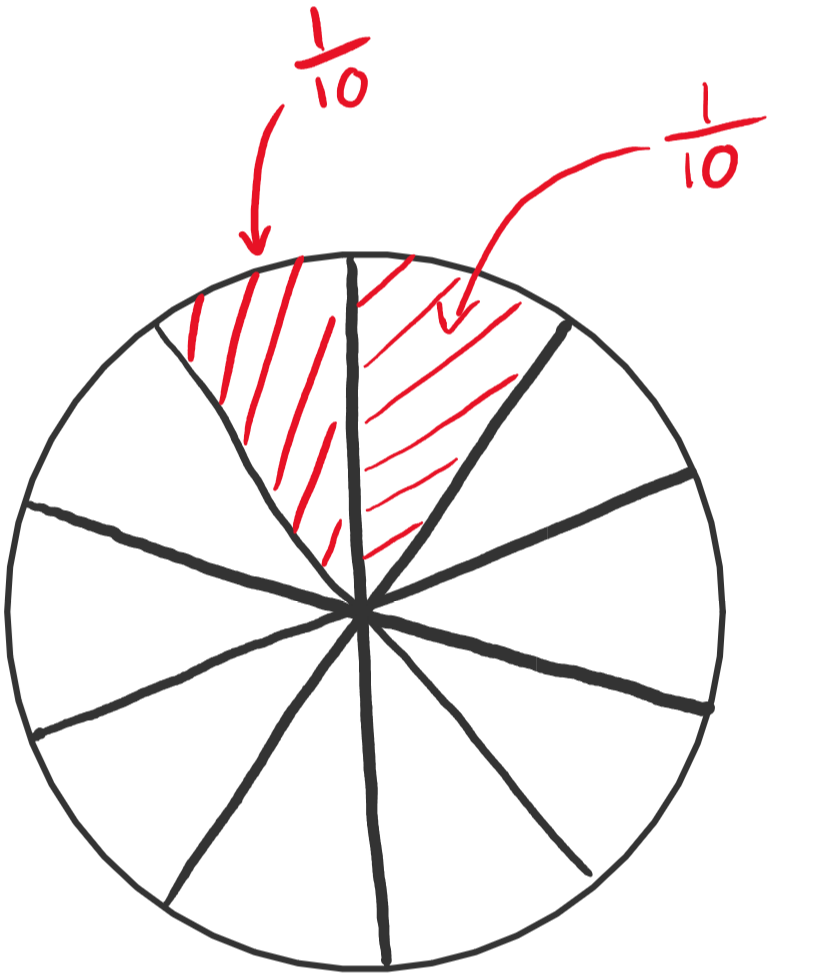
\includegraphics[scale=0.52]{chapter5_draw2.png}
\end{center}

Instead of just highlighting the one part, we highlight two. But what about as a number? Well we know we can use multiplication to represent multiple of something: 
\[ \frac{1}{10} \cdot 2 = \frac{1}{10} + \frac{1}{10} \]

But that feels hard to write that down every single time. So instead we have come up with a convention for notating this. We say: 
\[ \frac{1}{10} \cdot 2 = \frac{2}{10} \]

This number, $\frac{2}{10}$, can simply be thought of as $\frac{1}{10} \cdot 2$. But you can also think of it as splitting the number 2 into 10 groups. 
If you think about it, this is what we were doing with $\frac{1}{10}$. That number represented a part ten times smaller than 1.
Take a second to confirm to yourself that it makes sense that something that is ten times smaller than 2 is the same thing as two things that are both ten times smaller than 1. Or that this is true: 
\[ \frac{1}{10} \cdot 2 = \frac{2}{10} \]

\section*{Fractions, properly}

So we have gotten to halfway through the second page and I haven't even fully explained to you the title: Rational Numbers. 
So let me give you the most general definition of a rational number and we will then explore what it means. I am going to use two variables to represent two integers: $a$ and $b$ (they each can be any integer. So it could be that $a = 5$ and $b=9$ or $a=-2$ and $b=5$. Go back to the variables notes if this feels weird to you.)
If you remember, we think of integers as the following numbers: 
\[ \ldots -4, -3, -2, -1, 0, 1, 2, 3, 4, \ldots \]

Where of course we keep counting down in negative numbers and counting up with the positive numbers forever. We define a rational number to be any number that can be created like so: 
\[ \frac{a}{b} \]

But what does that value mean? Well, much like how we can write $\frac{2}{10} = \frac{1}{10} \cdot 2 = 2 \cdot \frac{1}{10}$ (remember we can reverse multiplication)
we can rewrite this in the same way: 
\[ \frac{a}{b} = a \cdot \frac{1}{b} \]

And we know what these values are! $a$ is just, well, $a$. It is just some integer. and $\frac{1}{b}$, well that is the multiplicative inverse of $b$! (Remember, this means: $b \cdot \frac{1}{b} = 1$)

We can think of multiplying $a$ by the multiplicative inverse of $b$ as splitting $a$ into $b$ parts. So that is all a rational number is. One integer which we have split into a certain number of parts. 

Now I am sure that doesn't entirely answer all of your questions about what a fraction is. I am introducing this to you very 
abstractly and you are in no way expected to entirely understand it right now. But, I do need to explain a few more things to you. For starters, I said that this was a rational number earlier: 
\[ 1 \]

But that doesn't look anything like: 
\[ \frac{a}{b} \]

There is only 1 number and there definitely isn't a horizontal bar... So what's up with that? Well, consider what $\frac{a}{b}$ means. All this is saying is we are splitting $a$ into $b$ parts. Well, what if we were keeping $a$, well then we would ``split'' it into 1 part... Or not split it at all. 
And so if we want to split it into just 1 group, so not split it at all, we can say $b=1$. And if we just want 1, well 1 split into 1 group is still 1. So we should have the fraction:
\[ 1 = \frac{1}{1} \]

And now that we understand how to do that, it should be pretty easy to see that if we have the number $c$, we can create a fraction to represent it like so: 
\[ c = \frac{c}{1} \]

\section*{Adding Fractions}
So we have already talked about adding fractions like this: 
\[ \frac{1}{10} + \frac{1}{10} \]

This should be: 
\[ \frac{2}{10} \]

We can see this through multiplication, but also if we think about it for a little bit. If we were to draw a diagram of this stiuation: 
\begin{center}
    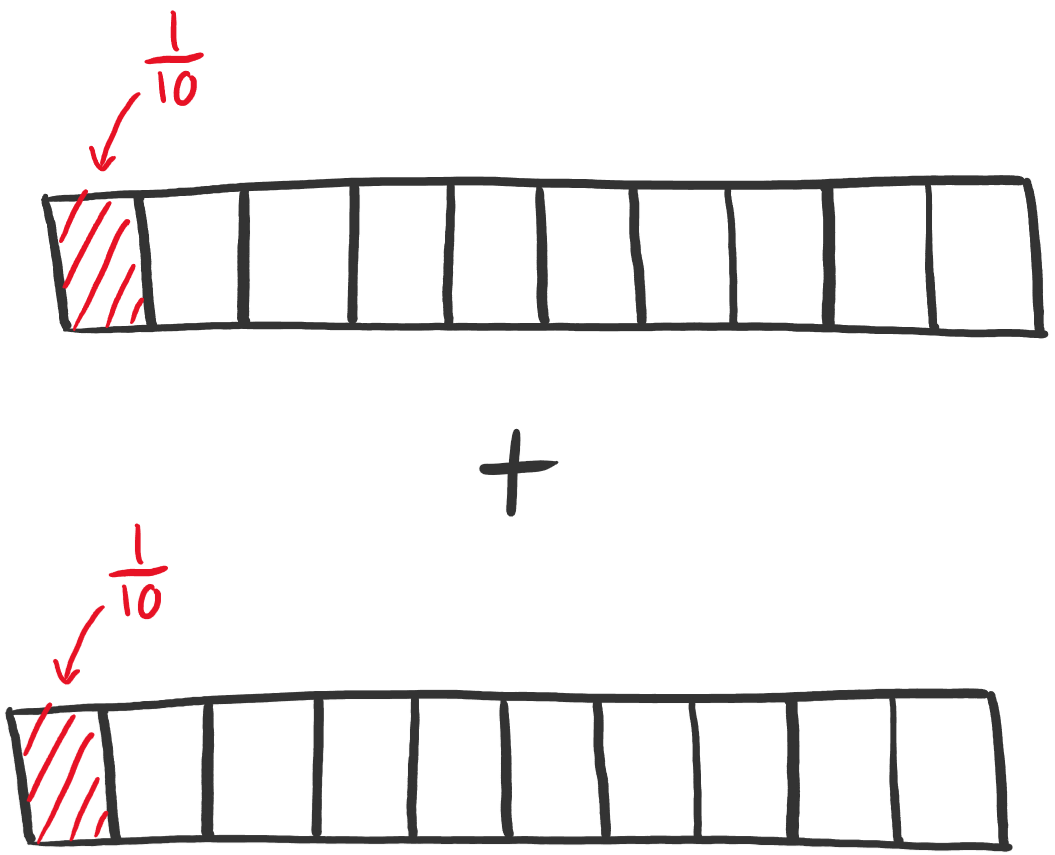
\includegraphics[scale=0.5]{chapter5_draw3.png}
\end{center}

In order to add the two parts together, we can include them on the same diagram: 
\begin{center}
    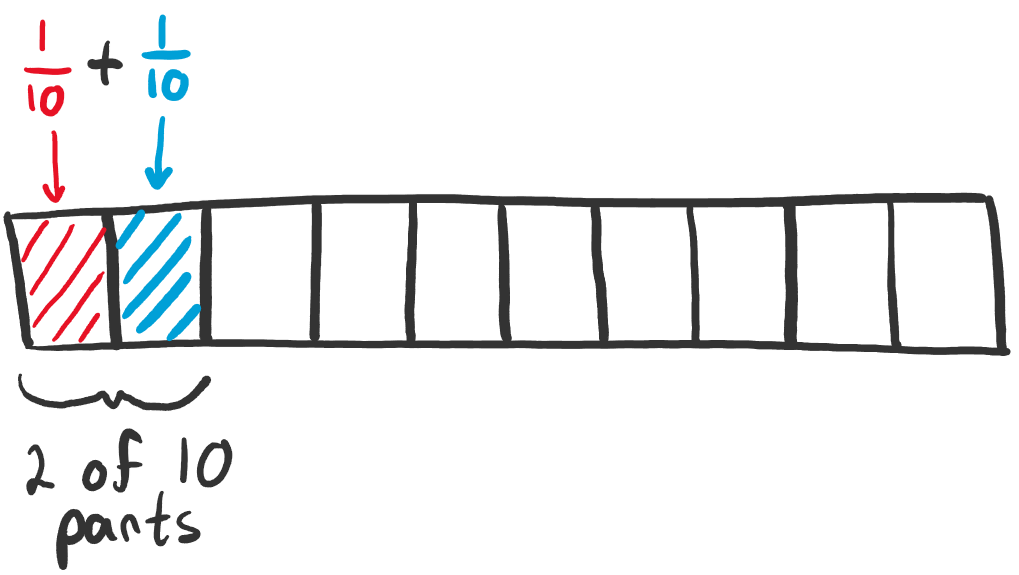
\includegraphics[scale=0.5]{chapter5_draw4.png}
\end{center}

And from this drawing, we can simply count how many of the ten parts are taken up. We find that 2 of them are filled up, meaning that we can say: 
\[ \frac{1}{10} + \frac{1}{10} = \frac{2}{10} \]

But now say we want to add two different fractions. Say: 
\[ \frac{1}{3} + \frac{1}{4} \]

How do we add these? If we were to draw a diagram of the situation: 
\begin{center}
    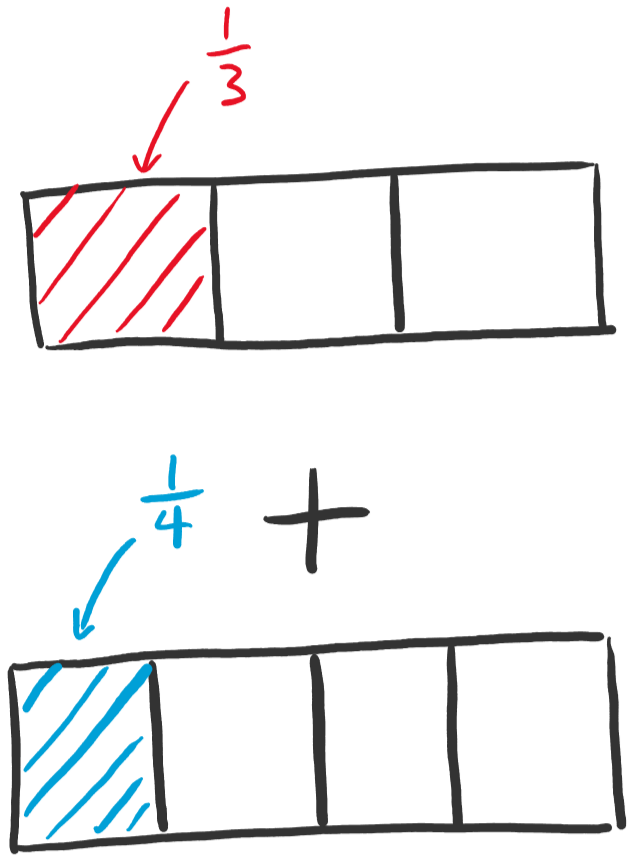
\includegraphics[scale=0.5]{chapter5_draw5.png}
\end{center}

We can't really combine these drawings like we did above, there are different numbers of partitions for the two objects. So then what can we do? 
This is something you will explore for homework! 

\section*{Multiplying Fractions}
How do we do multiplication with fractions? I mean, we have been using them like we can (and actually doing some multiplication with them), but we haven't really talked about how this works. Of course, we have said the following is true: 
\[ 2 \cdot \frac{1}{10} = \frac{2}{10} \]

And we have also said that $2 = \frac{2}{1}$, so this would suggest that we are saying: 
\[ \frac{2}{1} \cdot \frac{1}{10} = \frac{2}{10} \]

So here we are multiplying fractions, but it doesn't seem to tell us much about how we would do this for any fraction. We might make the connection that the new fraction is created like so: 
\[ \frac{2}{1} \cdot \frac{1}{10} = \frac{2 \cdot 1}{1 \cdot 10} = \frac{2}{10} \]

Which would suggest that for any two fractions, we would find: 
\[ \frac{a}{b} \cdot \frac{c}{d} = \frac{ac}{bd} \]

But this really isn't motivated by anything? How did we come to this conclusion? What does it mean? Of course I wouldn't have shown you this if it wasn't correct, but I want to actually explain this to you so here that goes. 

Say we split something into 4 parts. This would give us the fraction: $\frac{1}{4}$. One of 4 parts of the number 1. But now let's say we split that single part into three parts. Now what fraction do we have? 
Well the one thing we do know is that multiplying by $\frac{1}{3}$ is equivalent to splitting something into 3 parts. So we are looking for the following: 
\[ \frac{1}{4} \cdot \frac{1}{3} = \text{ ???} \] 

We can try and find an answer by creating another picture! (Pictures solve everything in math) We start by looking at something split into 4 parts: 
\begin{center}
    
\includegraphics[scale=0.7]{chapter5_draw6.png}
\end{center}

Taking just one of those 4 parts would be equivalent to $\frac{1}{4}$, just like what we have done before. But now, remember, we want to split each part into 3 more parts. So let's do that: 
\begin{center}
    
\includegraphics[scale=0.7]{chapter5_draw7.png}
\end{center}

And... Well, we want just one of those parts: 
\begin{center}
    
\includegraphics[scale=0.7]{chapter5_draw8.png}
\end{center}

And simply by counting, we can see that this one part is one-twelfth of the whole. Or the number: $\frac{1}{12}$. This also happens to follow our rule:
\[ \frac{1}{4} \cdot \frac{1}{3} = \frac{1\cdot 1}{4\cdot 3} = \frac{1}{12}  \]

And this makes sense, looking at the way we split the drawing up above, it looks very similar to multiplication. We created 4 groups of 3 things! Just like multiplication! 
But instead of taking all parts of that multiplication, we are just splitting something up into that many parts. Hence the rule: 
\[ \frac{1}{a} \cdot \frac{1}{b} = \frac{1}{ab}\]

I encourage you to explore this rule and convince yourself that it is true if you aren't already. Of course, we will explore this in class as well. 

But now, you probably want to ask, how can we fully calculate: 
\[ \frac{a}{b} \cdot \frac{c}{d} \]

Of course, I mentioned how to do this earlier, but I want you to be fully convinced as to how this works. So, take the above expression and split the fractions like so: 
\[ \left(a \cdot \frac{1}{b}\right) \cdot \left(c \cdot\frac{1}{d}\right) \]

What can we do with this? Well, we don't have to simplify anything in either expression, so we can just get rid of the parenthesis: 
\[ a \cdot \frac{1}{b} \cdot c \cdot \frac{1}{d} \]

And also remember, we can rearrange multiplication: 
\[ a \cdot c \cdot \frac{1}{b} \cdot \frac{1}{d} \]

Well, we know how to multiply $a \cdot c$! We have done that so many times! So we can simplify that: 
\[ \left(ac\right) \cdot \frac{1}{b} \cdot \frac{1}{d} \]

And we just found out how to multiply together the two fractions: 
\[ \left(ac\right) \cdot \left(\frac{1}{bd}\right) \]

And what does this look like? Well it looks just like: 
\[ \text{some number } \cdot \frac{1}{\text{some other number}} \]

Which we know how to simplify! We can write: 
\[ \frac{a}{b} \cdot \frac{c}{d} = \frac{ac}{bd} \]

Just like we guessed at the beginning! 

But that is probably more fractions then you ever wanted to see, so we will leave it there for now. 

\section*{Problems}
\begin{multicols*}{2}
    For problems 1-15, simplify the expression as much as possible. If you are unsure as to how to do it, try to theorize about how you might. Try a few things, see if they work!
    \begin{enumerate}
        \item $ \frac{1}{3} + \frac{1}{3}$
        \item $ \frac{3}{20} + \frac{4}{20} $
        \item $ \frac{1}{12} + \frac{4}{12} $
        \item $ \frac{3}{12} + \frac{4}{12} $
        \item $ \frac{1}{4} + \frac{1}{3} $
        \item $ \frac{1}{3} + 1 $
        \item $ \frac{3}{6} + \frac{1}{2} $
        \item $ \frac{1}{5} \cdot \frac{1}{2} $
        \item $ 4 \cdot \frac{1}{5} $
        \item $ 4 \cdot \frac{1}{4} $ 
        \item $ 25 \cdot \frac{1}{5} $
        \item $ \frac{2}{5} \cdot \frac{4}{6} $
        \item $ \frac{14}{20} \cdot \frac{12}{3} $
        \item $ \frac{3}{7} \cdot \frac{4}{9} $
        \item $ \frac{3}{12} + \frac{1}{4} $
        \item What can you say about the relationship between $\frac{1}{2}$ and $\frac{3}{6}$? Do they have any equivalence? Are they related in some other way?
        \item Are $\frac{2}{4}$ and $\frac{5}{10}$ the same thing? If so, why? If not, why not? 
        \item What is the multiplicative inverse of $\frac{4}{5}$? In other words, can you find $a$ in the following equation: $\frac{4}{5} \cdot a = 1$?
        \item Same as 18 but for $\frac{6}{7}$. 
        \item Same as 18 but for $\frac{1}{3}$. 
        \item What is the additive inverse of $\frac{1}{4}$? What about $\frac{1}{7}$? What about $\frac{7}{8}$? 
        \item What is the additive inverse of $\frac{a}{b}$? 
        \item What is the multiplicative inverse of $\frac{a}{b}$?
        \item Can you come up with a simplification of $\frac{1}{a} + \frac{1}{b}$? IE: make them into a single fraction? For any value of $a$ and $b$. 
        \item Is there a simpler way to write $\frac{32}{8}$? What about $\frac{25}{5}$? What about $\frac{10}{5}$? 
    \end{enumerate}
\end{multicols*}



\end{document}